\section{Механизмы, поддерживающие высокую готовность}

\begin{grayquote}
    \textbf{Высокая доступность (High Availability, HA)} - это характеристика технической системы, разработанная для избежания невыполненного обслуживания путём уменьшения или управления сбоями и минимизации времени плановых простоев \autocite{WikiHA}. Доступность часто измеряется в <<Nines>> (девятках), где каждый дополнительный девятый в проценте доступности существенно снижает допустимое время простоя системы.
\end{grayquote}

Высокая готовность для каждой конкретной системы зависит от цели, для которой предназначена эта система. Для некоторых организаций высокая готовность означает допустимое общее время простоя (downtime) за год в пределах нескольких минут. Для других систем приемлемым может быть суммарный downtime, достигающий нескольких часов в месяц \autocite{OszuValduriez}.
Важность понимания уровней доступности иллюстрируется на рисунке 4, где приведены значения допустимого времени простоя при различных уровнях HA:

\begin{center}
    \begin{tabular}{|l|c|c|c|c|c|}
        \hline
        \textbf{Availability \%} & \textbf{per year} & \textbf{per quarter} & \textbf{per month} & \textbf{per week} & \textbf{per day (24h)} \\
        \hline
        90\% ("one nine")       & 36.53 days  & 9.13 days   & 73.05 hours & 16.80 hours & 2.40 hours \\
        \hline
        95\% ("one nine five")  & 18.26 days  & 4.56 days   & 36.53 hours & 8.40 hours  & 1.20 hours \\
        \hline
        97\% ("one nine seven") & 10.96 days  & 2.74 days   & 21.92 hours & 5.04 hours  & 43.20 minutes \\
        \hline
        98\% ("one nine eight") & 7.31 days   & 43.86 hours & 14.61 hours & 3.36 hours  & 28.80 minutes \\
        \hline
        99\% ("two nines")      & 3.65 days   & 21.9 hours  & 7.31 hours  & 1.68 hours  & 14.40 minutes \\
        \hline
        99.5\% ("two nines five") & 1.83 days & 10.98 hours & 3.65 hours  & 50.40 minutes & 7.20 minutes \\
        \hline
        99.8\% ("two nines eight") & 17.53 hours & 4.38 hours & 87.66 minutes & 20.16 minutes & 2.88 minutes \\
        \hline
        99.9\% ("three nines")  & 8.77 hours  & 2.19 hours  & 43.83 minutes & 10.08 minutes & 1.44 minutes \\
        \hline
        99.95\% ("three nines five") & 4.38 hours & 65.7 minutes & 21.92 minutes & 5.04 minutes & 43.20 seconds \\
        \hline
        99.99\% ("four nines")  & 52.60 minutes & 13.15 minutes & 4.38 minutes & 1.01 minutes & 8.64 seconds \\
        \hline
    \end{tabular}
\end{center}

Как видно из таблицы, повышение доступности с 99\% до 99.9\% сокращает время простоя системы с нескольких дней до нескольких часов в год, что существенно влияет на требования к архитектуре, резервированию и восстановлению данных \autocite{RajeshKumar}.

Высокая готовность включает в себя несколько ключевых аспектов, среди которых выделяют:
\begin{itemize}
    \item Доступность данных
    \item Защиту данных
    \item Производительность
    \item Стоимость поддержки инфраструктуры
\end{itemize}

Каждый из этих аспектов требует комплексного подхода, начиная от проектирования аппаратной платформы и заканчивая настройкой программного обеспечения и организацией процессов мониторинга и администрирования \autocite{Kleppmann}.

\subsection{Средства, поддерживающие высокую готовность} ~\\

Обеспечение высокой готовности баз данных требует применения широкого спектра технических средств и архитектурных решений. Эти средства направлены на устранение единичных точек отказа, обеспечение непрерывной работы сервисов, автоматическое переключение на резервные ресурсы и минимизацию времени восстановления после сбоев \autocites{RajeshKumar}{SameerParadkar}.

Средства, поддерживающие высокую готовность, можно классифицировать следующим образом:
\begin{itemize}
    \item Аппаратные средства обеспечения высокой готовности;
    \item Программные средства обеспечения высокой готовности;
    \item Кластеризация серверов баз данных;
    \item Параметры настройки СУБД для повышения готовности;
    \item Средства резервного копирования и восстановления данных.
\end{itemize}

В последующих подразделах будут рассмотрены основные подходы и технологии в рамках каждого из перечисленных направлений, а также приведены практические примеры и иллюстрации.

%НИЖЕ ПОКА НЕ ТРОГАНО С 5.1.1.

\paragraph{Аппаратная и программная поддержки} ~\\
Существует несколько возможных уровней обеспечения высокой готовности системы: аппаратный и программный уровни. \\
\subsubsection{Аппаратные средства, поддерживающие высокую готовность}
\underline{Аппаратный уровень} включает в себя:
\begin{enumerate}
    \item \underline{Репликация БД}
    Репликация позволяет скопировать данные с одного сервера бд на другой.
    Существуют  два подхода репликации баз данных, рассмотрим каждый из них \autocite{Gregorchenko}:
    \begin{itemize}
        \item \underline{Репликация Master-Slave} \\В этом подходе выделяется один основной сервер базы данных, который называется Master. На нем происходят все изменения в данных (любые запросы INSERT/UPDATE/DELETE). Slave-сервер постоянно копирует все изменения с Master. С приложения на Slave-сервер могут отправляться запросы на чтение данных (запросы SELECT). Таким образом Master-сервер может отвечать за изменения данных, а Slave за чтение. Также Master сервер может отвечать за все операции с данными, а Slave являться бэкапом. При выходе из строя Slave, достаточно просто переключить все приложение на работу с Master. После этого восстановить репликацию на Slave и снова его запустить. Если выходит из строя Master, нужно переключить все операции (и чтения, и записи) на Slave. Таким образом он станет новым Master. После восстановления старого Master, настроить на нем реплику, и он станет новым Slave.
        Выше был рассмотрен случай асинхронной репликации. При синхронной репликации результат сразу же записывается и в Master, и в Slave. Возвращение управления клиенту происходит только после записи в обе базы.
        \item \underline{Репликация Master-Master}\\ В этой схеме любой из серверов может использоваться как для чтения, так и для записи. При использовании такого типа репликации достаточно выбрать случайного Master для обработки соединения, но часто один из серверов выбирается основным(Active), а другой(Passive) используется, как бэкап, в который при необходимости(в случае выхода из строя основного) можно легко начать писать данные. Репликация типа Мастер-Мастер для баз данных увеличивает скорость доступа к данным и повышает избыточность для действующих сайтов. Но данная схема обладает недостатком из-за возможных рассинхронизаций при записи данных. 
    \end{itemize}  

    Помимо разбиения репликаций по способу организации системы (см. выше) стоит выделить различные подходы по способу внесения изменений в базу данных. Рассмотрим на примере PostgreSQL, который поддерживает эти реализации \autocite{PostrgreSQL1}.
    \begin{itemize}
        \item \underline{Потоковая репликация} \\Это репликация, при которой от основного сервера PostgreSQL на реплики передается WAL(журнал предзаписи транзакций). И каждая реплика затем по этому журналу изменяет свои данные. Для настройки такой репликации все серверы должны быть одной версии, работать на одной ОС и архитектуре. Потоковая репликация в Postgres бывает двух видов — асинхронная и синхронная.
		\begin{enumerate}
        		\item{Асинхронная репликация} \\В этом случае PostgreSQL сначала применит изменения на основном узле и только потом отправит записи из WAL на реплики. Преимущество такого способа — быстрое подтверждение транзакции, т.к. не нужно ждать пока все реплики применят изменения. Недостаток в том, что при падении основного сервера часть данных на репликах может потеряться, так как изменения не успели продублироваться.
        		\item{Синхронная репликация} \\В этом случае изменения сначала записываются в WAL хотя бы одной реплики и только после этого фиксируются на основном сервере. Преимущество — более надежный способ, при котором сложнее потерять данные. Недостаток — операции выполняются медленнее, потому что прежде чем подтвердить транзакцию, нужно сначала продублировать ее на реплике.
        	\end{enumerate}
        	\item \underline{Логическая репликация} \\Логическая репликация оперирует записями в таблицах PostgreSQL. Этим она отличается от потоковой репликации, которая оперирует физическим уровнем данных: биты, байты, и адреса блоков на диске. Возможность настройки логической репликации появилась в PostgreSQL 10.
Этот вид репликации построен на механизме публикации/подписки: один сервер публикует изменения, другой подписывается на них. При этом подписываться можно не на все изменения, а выборочно. Например, на Master-сервере 50 таблиц: 25 из них могут копироваться на один Slave-сервер, а 25 — на другой.
Также есть несколько ограничений, главное из которых — нельзя реплицировать изменения структуры БД. То есть если на Master-сервере добавится новая таблица или столбец — эти изменения не попадут в Slave автоматически, их нужно применять отдельно.
В отличие от потоковой репликации, логическая может работать между разными версиями PostgreSQL, ОС и архитектурами.
	\end{itemize}
     \item \underline{RAID} - технология виртуализации данных для объединения нескольких физических дисковых устройств в логический модуль для повышения отказоустойчивости и производительности.
     Рассмотрим базовые уровни рейд массивов \autocite{Patterson}:
     \begin{enumerate}
         \item RAID 0 (striping — «чередование») — дисковый массив из двух или более жёстких дисков без резервирования. Информация разбивается на блоки данных фиксированной длины и записывается на оба/несколько дисков поочередно.
         \item RAID 1 (mirroring — «зеркалирование») — массив из двух (или более) дисков, являющихся полными копиями друг друга. Не следует путать с массивами RAID 1+0 (RAID 10), RAID 0+1 (RAID 01), в которых используются более сложные механизмы зеркалирования.
         \item RAID 2. Массивы такого типа основаны на использовании кода Хэмминга. Диски делятся на две группы: для данных и для кодов коррекции ошибок, причём если данные хранятся на $2 ^ n - n - 1$ дисках, то для хранения кодов коррекции необходимо $n$ дисков. Суммарное количество дисков при этом будет равняться $2 ^ n - 1$. Данные распределяются по дискам, предназначенным для хранения информации, так же, как и в RAID 0, то есть они разбиваются на небольшие блоки по числу дисков.
         \item В массиве RAID 3 из $n$ дисков данные разбиваются на куски размером меньше сектора (разбиваются на байты или блоки) и распределяются по $n - 1$ дискам. Ещё один диск используется для хранения блоков чётности. В RAID 2 для этой цели применялся $n - 1$ диск, но большая часть информации на контрольных дисках использовалась для коррекции ошибок «на лету», в то же время большинство пользователей устраивает простое восстановление информации в случае её повреждения, для чего хватает данных, умещающихся на одном выделенном жёстком диске. \\ Отличия RAID 3 от RAID 2: невозможность коррекции ошибок на лету.
         \item RAID 4 похож на RAID 3, но отличается от него тем, что данные разбиваются на блоки, а не на байты. Таким образом, удалось отчасти «победить» проблему низкой скорости передачи данных небольшого объёма. Запись же производится медленно из-за того, что чётность для блока генерируется при записи и записывается на единственный диск.
         \item RAID 5. Основным недостатком уровней RAID от 2-го до 4-го является невозможность производить параллельные операции записи, так как для хранения информации о чётности используется отдельный контрольный диск. RAID 5 не имеет этого недостатка. Блоки данных и контрольные суммы циклически записываются на все диски массива, нет асимметричности конфигурации дисков. Под контрольными суммами подразумевается результат операции XOR (исключающее или). XOR обладает особенностью, которая даёт возможность заменить любой операнд результатом, и, применив алгоритм XOR, получить в результате недостающий операнд.
         \item RAID 6 — похож на RAID 5, но имеет более высокую степень надёжности — два (или более) диска данных и два диска контроля чётности. Основан на кодах Рида — Соломона и обеспечивает работоспособность после одновременного выхода из строя любых двух дисков. Обычно использование RAID 6 вызывает примерно 10-15 \% падение производительности дисковой группы, относительно RAID 5, что вызвано б\'{о}льшим объёмом работы для контроллера (более сложный алгоритм расчёта контрольных сумм), а также необходимостью читать и перезаписывать больше дисковых блоков при записи каждого блока.
     \end{enumerate}
     Также существуют различные комбинации данных подходов.
\end{enumerate}

\subsubsection{Программные средства, поддерживающие высокую готовность} ~\\
\underline{Программные подходы}:
\begin{enumerate}
    \item \underline{Автоматический перезапуск экземпляров БД, сетевых демонов и других ресурсов}
    \item \underline{Защита от повреждения данных(Data corruption protection)}
    \begin{itemize}
        \item Использование контрольных чек-сумм
        \item Автоматическое восстановление из резервной копии или повторная передача
    \end{itemize}
    \item \underline{PITR (Point In Time Recovery)} это технология, используемая в базах данных для восстановления данных на конкретный момент времени. Эта функция необходима для восстановления после случайного удаления данных, их повреждения или других непредвиденных проблем. Вот краткое описание работы PITR и её преимуществ:
    \begin{itemize}
        \item Непрерывное резервное копирование: \\
        PITR включает непрерывное резервное копирование журналов транзакций базы данных, помимо регулярных полных резервных копий. Эти журналы транзакций фиксируют каждое изменение, сделанное в базе данных, что позволяет точно восстановить данные.
        \item Процесс восстановления: \\
        Для выполнения PITR необходимо начать с последней полной резервной копии, а затем применить журналы транзакций до желаемого момента времени. Этот момент может быть любым до возникновения повреждения или потери данных.
        \item Гибкость и точность: \\
        Этот метод позволяет очень точно восстановить данные, вплоть до конкретной минуты или даже секунды, в зависимости от частоты логирования. Это особенно полезно для минимизации потерь данных во время восстановления.
        \item Сценарии использования: \\
        PITR идеально подходит для восстановления после ошибок пользователя, таких как случайное удаление или изменение данных, а также после определённых видов повреждения данных. Эта технология позволяет отменить нежелательные изменения без значительных потерь данных.
        \item Реализация: \\
        Различные системы баз данных реализуют PITR по-разному. Например, PostgreSQL использует Write-Ahead Logging (WAL) для PITR, где файлы WAL содержат необходимую информацию для восстановления состояния базы данных. Oracle, MySQL и SQL Server имеют свои собственные методы обработки журналов транзакций и выполнения PITR.
    \end{itemize}
    \item \underline{Application continuity (Oracle)} \cite{availability-ApplicationContinuity} это технология, разработанная для повышения надежности и устойчивости работы приложений при сбоях. Она позволяет приложениям автоматически восстанавливать выполнение транзакций, минимизируя влияние на конечных пользователей. Вот основные аспекты этой технологии:
    \begin{itemize}
        \item Непрерывность транзакций: \\
        Application Continuity обеспечивает автоматическое повторное выполнение транзакций после сбоев. Это означает, что при сбое соединения с базой данных или при перезагрузке сервера транзакции продолжаются с того места, где они были прерваны, без необходимости вмешательства пользователя.
        \item Механизм работы: \\
        Технология сохраняет состояние транзакции и контекст выполнения, а затем использует эти данные для восстановления и повторного выполнения операций. Это включает в себя сохранение всех вызовов SQL и PL/SQL, которые приложение выполняло до сбоя.
        \item Прозрачность для пользователей: \\
        Пользователи не замечают сбоев, так как восстановление происходит прозрачно для них. Это обеспечивает высокую степень удовлетворенности пользователей и повышает доверие к системе.
        \item Интеграция и использование: \\
        Application Continuity интегрируется с Oracle Database и поддерживается в различных архитектурах, включая Oracle Real Application Clusters (RAC) и Oracle Active Data Guard. Это позволяет использовать технологию в масштабируемых и распределенных системах.
        \item Преимущества: \\
        Основные преимущества включают снижение риска потери данных, повышение доступности приложений и улучшение пользовательского опыта. Технология помогает обеспечить высокие уровни SLA (Service Level Agreement) за счет минимизации простоев.
    \end{itemize}
    \item \underline{WAL} Данный подход будет описан ниже.
\end{enumerate}

\subsubsection{Кластерная организация серверов баз данных} ~\\

Кластеризация базы данных - это процесс объединения нескольких серверов или инстансов, соединяющих одну базу данных. Иногда одного сервера может быть недостаточно для управления объемом данных или количеством запросов, тогда возникает необходимость в кластере. 
 
К общим требованиям, предъявляемым к кластерным системам, относятся:
\begin{enumerate}
    \item Высокая готовность
    \item Высокое быстродействие
    \item Масштабирование
    \item Удобство обслуживания
\end{enumerate}

Кластеры баз данных являются распространенной технологией.  Рассмотрим три типа архитектуры кластерных вычислений. Отказоустойчивые кластеры, высокопроизводительные кластеры и кластеры балансировки нагрузки.

\begin{enumerate}
\item Отказоустойчивые / высокодоступные кластеры. Кластер обеспечивает доступность сервиса путем репликации серверов и избыточной реконфигурации программного и аппаратного обеспечения. Таким образом, каждая система контролирует другую и работает на запросы, если какой-либо один из узлов выходит из строя.

\item Высокопроизводительные кластеры. Целью разработки высокопроизводительных кластеров баз данных является создание высокопроизводительных компьютерных систем. Основная цель - разумное распределение рабочей нагрузки.

\item Кластеры балансировки нагрузки. Эти кластеры базы данных служат для распределения нагрузки между различными серверами. Они стремятся обеспечить увеличенную пропускную способность сети, в конечном итоге увеличивая производительность. Системы в этой сети объединяют свои узлы, с помощью которых пользовательские запросы равномерно распределяются между участвующими узлами.
\end{enumerate}

Несмотря на всю распределенную систему на заднем плане, пользователю это кажется единой системой. Использование кластеров варьируется от предприятия к предприятию, в зависимости от вида процессов и требуемого уровня производительности.
\subsubsection{Параметры настройки СУБД}
Для обеспечения высокой доступности (HA) в системах управления базами данных (СУБД) необходимо правильно настроить различные параметры. Вот основные параметры настройки, относящиеся к HA, на примере таких СУБД как PostgreSQL, Oracle и MySQL:
\paragraph{PostgreSQL} \cite{availability-postgres}
\begin{enumerate}
    \item Streaming Replication:
    \begin{itemize}
        \item wal\_level: Установите значение replica для включения репликации.
        \item max\_wal\_senders: Указывает максимальное количество процессов отправки WAL (Write-Ahead Logging).
        \item wal\_keep\_segments: Определяет, сколько сегментов WAL следует сохранять для репликации.
        \item archive\_mode и archive\_command: Включите архивирование WAL для обеспечения PITR (Point-In-Time Recovery).
    \end{itemize}
    \item Hot Standby:
    \begin{itemize}
        \item hot\_standby: Установите on, чтобы разрешить выполнение запросов на репликах.
        \item max\_standby\_streaming\_delay: Задает максимальную задержку для потоковой реплики перед откатом длительных транзакций.
    \end{itemize}
    \item Failover: Используйте инструменты, такие как Patroni, pg\_auto\_failover или repmgr, для автоматического переключения на резервный сервер при сбое основного.
\end{enumerate}
\paragraph{Oracle} \cite{availability-oracle}
\begin{enumerate}
    \item Oracle Real Application Clusters (RAC):
    \begin{itemize}
        \item Cluster Interconnect: Настройте высокоскоростную сеть для обмена данными между узлами кластера.
        \item Instance Caging: Ограничьте ресурсы CPU для каждого экземпляра в кластере.
    \end{itemize}
    \item Data Guard:
    \begin{itemize}
        \item Redo Transport Services: Настройте передачу журналов redo на резервные серверы.
        \item Standby Redo Logs: Настройте резервные журналы redo для повышения производительности репликации.
        \item Data Guard Broker: Используйте для управления и автоматизации процессов Data Guard.
    \end{itemize}
    \item Flashback Technology:
    \begin{itemize}
        \item db\_flashback\_retention\_target: Установите цель времени для хранения данных Flashback.
        \item undo\_retention: Настройте для обеспечения длительных операций отката.
    \end{itemize}
\end{enumerate}
\paragraph{MySQL} \cite{availability-mysql}
\begin{enumerate}
    \item Replication:
    \begin{itemize}
        \item server\_id: Уникальный идентификатор сервера для репликации.
        \item log\_bin: Включите бинарные логи для записи всех изменений.
        \item binlog\_format: Установите формат бинарного лога (например, ROW для строковой репликации).
        \item relay\_log: Определите журналы ретрансляции для реплики.
    \end{itemize}
    \item Group Replication:
    \begin{itemize}
        \item group\_replication\_group\_name: Уникальное имя группы репликации.
        \item group\_replication\_start\_on\_boot: Автоматически запускать репликацию при запуске сервера.
        \item group\_replication\_bootstrap\_group: Используйте для инициализации группы.
    \end{itemize}
    \item High Availability Tools:
    \begin{itemize}
        \item Используйте MySQL InnoDB Cluster, ProxySQL и MHA (Master High Availability Manager) для автоматизации failover и балансировки нагрузки.
    \end{itemize}
\end{enumerate}

% НИЖЕ С 5.1.5 ИЗМЕНЕНИЯ ЕСТЬ

\subsubsection{Сохранение и восстановление БД} ~\\

Основным свойством транзакций СУБД является durability. Идея механизма обеспечения этого свойства является одинаковой для всех СУБД \autocite{PostrgreSQL1}. СУБД использует специальный механизм журналирования изменений.
Следовательно, с точки зрения файловой системы INSERT и UPDATE не являются атомарными операциями: если кто-то внезапно выключит ваш сервер, данные окажутся испорчены. Если возникает сбой, база данных использует этот файл для того, чтобы восстановить данные на момент падения. WAL -- это бинарный лог, так что для его чтения нужна специальная утилита.
Например в PostreSQL данный файл называется WAL и лежит по пути \$PGDATA/pg\_xlog.
PostgreSQL позволяет отключать WAL для отдельных таблиц, помечая их как UNLOGGED.

Дополнительно стоит отметить, что технологии журналирования WAL (Write-Ahead Logging) применяются не только PostgreSQL, но и других современных СУБД. Например, в Oracle Database аналогичный механизм реализуется через redo logs, в Microsoft SQL Server — через transaction logs. Эти журналы записывают все изменения данных до их фактической фиксации в основном хранилище и позволяют СУБД обеспечивать восстановление данных до последнего сохранённого состояния в случае внезапного сбоя системы \autocite{OszuValduriez}.
Также в современных реализациях WAL поддерживаются функции создания контрольных точек (checkpointing), которые позволяют ускорить процесс восстановления за счёт периодической фиксации согласованного состояния базы данных. Контрольные точки минимизируют объём журнала, который необходимо применять при восстановлении и снижают время простоя при перезапуске системы \autocite{GarciaMolina}.
Кроме того, в высоконагруженных средах часто используется технология непрерывной архивации WAL (continuous archiving). Она обеспечивает сохранение полного журнала всех транзакций во внешнее хранилище, что позволяет восстанавливать базу данных не только до последней контрольной точки, но и до произвольного момента времени между точками сохранения (point-in-time recovery) \autocite{Bernstein}. 
Это особенно важно если недопустима потеря даже минимального объёма данных.
То есть механизм WAL в совокупности с контрольными точками и архивацией обеспечивает надёжное сохранение целостности данных и основу для дальнейшего восстановления после аварийных сбоев в большинстве современных СУБД.


\subsubsection{Автоматизация восстановления в СУБД} ~\\

Современные СУБД для обеспечения высокой готовности зачастую используют механизмы автоматического восстановления после сбоев (self-healing mechanisms). Основная их цель заключается в минимизации времени простоя за счёт автоматического реагирования на отказ компонентов без вмешательства админа \autocite{SameerParadkar}.
Основными задачами автоматизации восстановления являются:
\begin{itemize}
    \item Обнаружение отказа сервера или узла базы данных
    \item Перезапуск или автоматическое переключение (failover) на резервный экземпляр
    \item Репликация актуального состояния данных на новые или восстановленные узлы
    \item Интеграция с системами мониторинга для координации процессов восстановления
\end{itemize}

Одной из базовых технологий автоматического восстановления является механизм автоматического failover в кластерах СУБД. Например, в кластерах PostgreSQL с использованием Patroni отказ основного узла автоматически инициирует выбор нового мастера на основе состояния реплик \autocite{Kleppmann}. В аналогичных системах на базе Oracle RAC переключение между узлами осуществляется через встроенный механизм Clusterware \autocite{OracleRAC}.
В средах, использующих контейнеризацию и оркестрацию (например Kubernetes) автоматизация восстановления обеспечивается через контроллеры ReplicaSet и StatefulSet. При обнаружении сбоя контейнера или узла система автоматически развёртывает новый экземпляр базы данных на другом доступном узле, сохраняя при этом состояние и целостность данных.
На уровне облачных платформ автоматическое восстановление входит в стандартные функции управляемых СУБД-сервисов. Так, в Amazon RDS Multi-AZ или Google Cloud SQL при обнаружении отказа происходит автоматическое переключение на синхронную реплику в другом дата-центре без потери соединения с приложениями \autocite{AmazonRds2}.
Применение self-healing технологий требует соблюдения нескольких условий. Ниже они перечислены:
\begin{itemize}
    \item Наличие настроенных механизмов репликации и синхронизации данных;
    \item Использование надёжных систем обнаружения отказов (watchdogs);
    \item Минимизация времени восстановления (RTO) и допустимой потери данных (RPO);
    \item Тестирование сценариев автоматического переключения и восстановления.
\end{itemize}


\subsection{Оперативное администрирование} ~\\

Оперативное администрирование включает в себя мониторинг состояния оборудования и программных компонентов, своевременное обнаружение и устранение сбоев, обеспечение восстановления после аварийных ситуаций, а также регулярное тестирование готовности системы к отказам \autocites{SameerParadkar}{heycoachHAA}.

Основной целью оперативного администрирования является поддержание непрерывной работоспособности БД засчет минимизации времени реакции на возникновение инцидентов и реализации механизмов быстрого переключения на резервные ресурсы.

Среди основных задач оперативного администрирования можно выделить следующие:
\begin{itemize}
    \item Регулярный мониторинг состояния серверов бд, сетевых компонентов и систем хранения данных
    \item Оперативное обнаружение и классификация сбоев оборудования или программного обеспечения
    \item Управление аварийным переключением сервисов (failover) на резервные узлы
    \item Контроль за актуальностью резервных копий данных и возможность их быстрого восстановления
    \item Управление политиками безопасности для защиты от НСД
    \item Проведение регулярных тестирований отказоустойчивости системы (disaster recovery tests) \autocite{Kleppmann}.
\end{itemize}

Эффективное оперативное администрирование требует использования специализированных программных средств мониторинга и автоматизированного управления событиями (такие как Zabbix, Prometheus, Nagios), или встроенные решения в крупных СУБД, таких как Oracle Enterprise Manager или SQL Server Management Studio.
На сегодняшний день к требованиям для систем оперативного администрирования относятся:
\begin{itemize}
    \item Возможность централизованного сбора и анализа событий в реальном времени
    \item Поддержка механизмов уведомлений об инцидентах (email, SMS, push-уведомления)
    \item Интеграция с системами автоматизированного реагирования и устранения неисправностей
    \item Поддержка аналитики для прогнозирования потенциальных отказов на основе исторических данных \autocite{Afonin}
\end{itemize}




\subsubsection{Задачи, средства и режимы администрирования} ~\\

Задачи администратора баз данных могут незначительно отличаться в зависимости от вида применяемой СУБД, но в основные задачи входит:
\begin{itemize}
    \item \textbf{Проектирование базы данных}. Включает в себя разработку структуры хранения данных, создание схем, определение индексов и ограничений, обеспечивающих целостность информации \autocite{GarciaMolina}
    \item \textbf{Оптимизация производительности базы данных}. Направлено на настройку запросов, конфигурацию параметров сервера и построение эффективных планов выполнения операций для минимизации времени отклика и снижения нагрузки на систему \autocite{OszuValduriez}
    \item \textbf{Резервирование и восстановление базы данных}. Включает в себя планирование процедур регулярного создания резервных копий, организацию аварийного восстановления при сбоях и разработку стратегий обеспечения непрерывности бизнеса (Business Continuity Planning) \autocite{Bernstein}
    \item \textbf{Обеспечение целостности баз данных}. Предусматривает контроль целостности схем, управление транзакциями, мониторинг сбоев и их последствий, а также применение процедур валидации и проверки данных на уровне приложений и СУБД
    \item \textbf{Обеспечение перехода на новую версию СУБД}. Связано с планированием миграции данных, тестированием совместимости приложений, обновлением системного ПО, минимизацией рисков связанных модернизацией инфраструктуры
\end{itemize}

Существует множество программных средств и способов администрирования БД, зависящих напрямую от типа используемой СУБД. Основным инструментом работы с базой данных является использование языка запросов DSL (Domain-Specific Language), а также специализированных программных комплексов. Например, для работы с СУБД Oracle широко применяется инструмент SQL Developer. Он позволяет управлять структурой базы данных, выполнять запросы, администрировать пользователей и проводить миграцию данных \autocite{SQLDeveloper}

Однако существуют и программы, поддерживающие работу с различными СУБД, например продукты компании JetBrains (например DataGrip), которые обеспечивают платформу для администрирования различных типов баз данных через единый интерфейс.

Отдельную категорию составляют средства мониторинга серверов баз данных, такие как Zabbix, Prometheus, Nagios и другие, которые обеспечивают непрерывный контроль состояния систем, отправляют уведомления об отклонениях и позволяют вовремя реагировать на возможные инциденты \autocite{SameerParadkar}.

%5.2.2 ниже не тронуто

\subsubsection{Мониторинг серверов СУБД} ~\\
Мониторинг СУБД можно условно разделить на два типа:
\begin{enumerate}
    \item Мониторинг средствами СУБД
    \item Мониторинг хостов и сервисов, на которых запущена БД.
\end{enumerate}
\underline{Мониторинг средствами СУБД} \\ Средства мониторинга, предоставляемые СУБД зависят в первую очередь от конкретной реализации этой системы, однако можно выделить метрики, которые в большинстве случаев собираются встроенным мониторингом. В первую очередь это объем операций ввода/вывода, необходимых для исполнения транзакции, утилизация процессоров и временем отклика системы. Наиболее распространенной метрикой оценки производительности системы является ее время отклика, которое представляет собой интервал времени, в течении которого сервер возвращает первую строку результата исполнения запроса, т.е. пользователь получает визуальное подтверждение того, что его запрос исполняется. Пропускная способность обслуживаемых сервером процессов и пользователей определяет сколько запросов возможно исполнить в фиксированный интервал времени, и сколько строк и какого размера возвращается клиенту. При увеличении числа активных процессов и/или пользователей, возрастает и их конкуренция за системные ресурсы. Результатом такой чрезмерной нагрузки может стать увеличение времени отклика и снижение общей пропускной способности. Большое влияние на производительности базы данных оказывает также физическая и логическая целостность данных. \\
\underline{Мониторинг хостов и сервисов, на которых запущена БД} \\ Рассмотрим две системы - немного устаревший, но еще использующийся Zabbix и более современный и активно набирающий популярность Prometheus \autocite{Prometheus-vs-Zabbix}.
\begin{itemize}

	\item \underline{Zabbix}\\ Многофункциональным средством является Zabbix — свободная система мониторинга и отслеживания статусов разнообразных сервисов компьютерной сети, серверов и сетевого оборудования. Он поддерживает несколько видов мониторинга. Simple checks — может проверять доступность и реакцию стандартных сервисов, таких как SMTP или HTTP без установки какого-либо программного обеспечения на наблюдаемом хосте. Zabbix agent — может быть установлен на UNIX-подобных или Windows хостах для получения данных о нагрузке процессора, использования сети, дисковом пространстве и так далее. External check — выполнение внешних программ. 
	С точки зрения пользователя Zabbix разделен на две большие части: сервер и агенты. Сервер расположен на одной машине, которая собирает и хранит статистические данные, а агенты располагаются на тех машинах, с которых собираются данные. Агенты Zabbix поддерживают как пассивные (polling), так и активные проверки (trapping). Пассивные проверки означают, что сервер Zabbix запрашивает значение у агента Zabbix, а агент обрабатывает запрос и возвращает значение серверу Zabbix. Активные проверки означают, что агент Zabbix запрашивает список активных проверок с сервера Zabbix, а затем периодически отправляет результаты.
	Важной особенностью Zabbix является способ хранения данных. Для своей работы данное средство при установке требует подключения внешней базы данных (MySQL, PostgreSQL, Oracle и т.д.).
	Также стоит отметить, что Zabbix не так гибок в запросах. Он использует ключи элементов для получения метрик.
	\item \underline{Prometheus}\\ Prometheus — это система мониторинга с открытым исходным кодом, предоставляющая своим пользователям мощный язык запросов, функции хранения и визуализации. Он собирает метрики в реальном времени и записывает их в базу данных временных рядов. Prometheus предоставляет многомерную модель данных, которая позволяет определять метрики по именам и/или тегам, чтобы идентифицировать их как часть уникального временного ряда. Благодаря большому сообществу многие сервисы могут отправлять метрики в формате Prometheus. Если какие-то сервисы не могут этого сделать, то есть множество библиотек, помогающих в экспорте существующих метрик из сторонних систем в виде метрик Prometheus. 
	Prometheus для хранения данных использует свою базу данных временных рядов (TSDB). Используя собственную TSDB, Prometheus может получать и обрабатывать несравненно больше метрик, чем многие другие системы мониторинга. Данные могут быть записаны даже с отметками времени с миллисекундным разрешением. 
	В отличие от Zabbix Prometheus является более гибким в плане выполнения запросов. Prometheus предоставляет собственный функциональный язык для запросов, который называется PromQL (Prometheus Query Language). PromQL невероятно гибкий, простой и мощный. Он может применять функции и операторы к вашим запросам метрик, фильтровать, группировать по меткам и использовать регулярные выражения для улучшения сопоставления и фильтрации.
\end{itemize} 

%5.2.3 ниже написано

\subsubsection{Планирование аварийного восстановления (Disaster Recovery Planning)} ~\\

Планирование аварийного восстановления (Disaster Recovery Planning, DRP) является важной составляющей стратегии обеспечения высокой готовности информационных систем. DRP охватывает разработку, документирование и тестирование процедур, которые должны быть выполнены для восстановления работы баз данных и связанных с ними сервисов после возникновения серьёзных инцидентов \autocite{SnedakerS}.

Целью планирования аварийного восстановления является минимизация времени простоя (Recovery Time Objective, RTO) и объема возможных потерь данных (Recovery Point Objective, RPO) при возникновении отказов инфраструктуры, программных сбоев или катастрофических событий наподобие стихийных бедствий, кибератак, масштабных сбоев питания \autocite{Kleppmann}.

Основные этапы разработки плана аварийного восстановления включают:
\begin{itemize}
    \item Идентификацию критичных систем, сервисов и баз данных, требующих защиты
    \item Оценку рисков и потенциальных последствий различных сценариев отказов
    \item Определение допустимых уровней времени восстановления (RTO) и потерь данных (RPO) для каждого критичного компонента
    \item Разработку детальных процедур восстановления: порядок действий, ответственные лица, используемые средства и инструменты
    \item Обеспечение наличия актуальных резервных копий данных и их регулярного тестирования
    \item Настройку альтернативных площадок восстановления (например, горячий, тёплый или холодный резервный дата-центр) \autocite{RajeshBasa}
    \item Организацию системы уведомления и координации действий персонала в случае наступления аварийной ситуации
\end{itemize}
Эффективный план аварийного восстановления должен быть не только разработан, но и регулярно тестироваться в рамках учений по восстановлению (Disaster Recovery Drills). Это позволяет выявить слабые места в существующих процедурах и обеспечить готовность персонала действовать \autocite{WallaceWebber}.
В современных облачных инфраструктурах DRP часто включает использование геораспределённых сервисов (Multi-Region Deployments) и автоматизированных систем резервного копирования и восстановления. Например в Amazon Web Services или Microsoft Azure реализованы средства для создания автоматических резервных копий и развертывания восстановленных экземпляров баз данных в альтернативных регионах \autocite{AmazonRds}.

%Ниже правится 5.3
\subsection{Функциональная насыщенность СУБД} ~\\

Функциональная насыщенность СУБД является одним из факторов их способности поддерживать высокую готовность и устойчивость к сбоям. Под функциональной насыщенностью понимается наличие в СУБД встроенных механизмов, направленных на обеспечение непрерывности работы, защиты данных, восстановления после сбоев и эффективности обработки больших объёмов транзакций \autocite{OszuValduriez}
В системах предназначенных для реализации высокой готовности достигается не только надёжность аппаратной платформы, но и комплексная поддержка программных функций, обеспечивающих избыточность, резервирование, масштабируемость, автоматическое восстановление и мониторинг. Без наличия соответствующих функций СУБД даже самая устойчивая аппаратная инфраструктура не может гарантировать требуемого уровня доступности \autocite{Kleppmann}
К основным аспектам функциональной насыщенности СУБД, влияющим на её способность обеспечивать высокую готовность, относятся:

\begin{itemize}
    \item поддержка репликации данных в режиме реального времени
    \item наличие встроенных механизмов резервного копирования и восстановления
    \item возможности для работы в кластерных и распределённых конфигурациях
    \item обеспечение масштабируемости без остановки работы систем
    \item поддержка механизмов контроля целостности и автоматической синхронизации данных
    \item наличие инструментов мониторинга состояния систем и управления отказами
\end{itemize}

Высокая функциональная насыщенность СУБД позволяет минимизировать человеческий фактор в процессе управления системой и автоматизировать процессы обеспечения отказоустойчивости.
В последующих подразделах будут рассмотрены различные формы избыточности, их классификация, а также роль аппаратной и программной избыточности в формировании надёжной архитектуры баз данных.

\subsubsection{Формы избыточности} ~\\
Системы, обеспечивающие непрерывный (fault tolerant) или почти непрерывный (high availability) доступ к данным обычно опираются на различные формы избыточности.
Как правило, это системы дублирования аппаратного обеспечения и контролируемой избыточности данных \autocite{Baron}.

Избыточность в высокодоступных системах может быть классифицирована следующим образом:

\begin{itemize}
    \item Аппаратная избыточность заключается в резервировании ключевых компонентов инфраструктуры, таких как серверы, сетевые адаптеры, накопители данных. При отказе одного из элементов система автоматически переключается на резервный компонент, что минимизирует время простоя \autocites{RajeshKumar}{heycoachHAA}.
    \item Программная избыточность реализуется через механизмы репликации данных, кластеризацию серверов баз данных и автоматическое восстановление сервисов. Такие технологии позволяют сохранить целостность и доступность данных даже при сбоях отдельных узлов \autocite{OszuValduriez}.
    \item Избыточность на уровне данных предполагает хранение копий информации в различных локациях или форматах. Это обеспечивает защиту от потери данных и даёт возможность быстро восстановить их в случае аварии \autocite{Kleppmann}.
    \item Сетевая избыточность обеспечивается за счёт использования нескольких сетевых путей и резервных каналов передачи данных. Это позволяет поддерживать доступность системы даже при частичном выходе сетевой инфраструктуры из строя \autocites{RajeshKumar}{heycoachHAA}.
\end{itemize}
Выбор оптимального сочетания различных форм избыточности зависит от требований к доступности системы, допустимого уровня потерь данных и доступных ресурсов. Эффективное управление избыточностью позволяет минимизировать риски потери данных и существенно повысить надёжность систем \autocite{OszuValduriez}.

\paragraph{Избыточность данных} ~\\
Нормальная форма — свойство отношения в реляционной модели данных, характеризующее его с точки зрения избыточности, потенциально приводящей к логически ошибочным результатам выборки или изменения данных. Нормальная форма определяется как совокупность требований, которым должно удовлетворять отношение.

Процесс преобразования отношений базы данных к виду, отвечающему нормальным формам, называется нормализацией. Нормализация предназначена для приведения структуры БД к виду, обеспечивающему минимальную логическую избыточность, и не имеет целью уменьшение или увеличение производительности работы или же уменьшение или увеличение физического объёма базы данных. Конечной целью нормализации является уменьшение потенциальной противоречивости хранимой в базе данных информации. Как отмечает К. Дейт,общее назначение процесса нормализации заключается в следующем:
\begin{itemize}
    \item исключение некоторых типов избыточности;
    \item устранение некоторых аномалий обновления;
    \item разработка проекта базы данных, который является достаточно «качественным» представлением реального мира, интуитивно понятен и может служить хорошей основой для последующего расширения;
    \item упрощение процедуры применения необходимых ограничений целостности.
\end{itemize}

Устранение избыточности производится, как правило, за счёт декомпозиции отношений таким образом, чтобы в каждом отношении хранились только первичные факты (то есть факты, не выводимые из других хранимых фактов). \\

\paragraph{Аппаратная избыточность} ~\\
Аппаратная избыточность может включать платформы с полным резервированием, поддерживающие (standby) процессоры, диски с двойным интерфейсом (dual-port), дисковые массивы и пр. Один из вариантов - зеркалирование дисков, когда один диск используется в качестве копии другого и может быть использован при сбое вместо него. Хотя аппаратная избыточность и важна для повышения общей надежности системы, ее реализация, как правило, не ориентирована на обработку транзакций СУБД и на связанные с этим специфические ограничения, например, обеспечение атомарности транзакции. В результате СУБД не может воспользоваться преимуществами чисто аппаратных решений резервирования cистемы для повышения своей производительности.

\paragraph{Программная избыточность} ~\\
Программная избыточность достигается за счёт дублирования программных компонентов и сервисов, обеспечивающих функционирование баз данных и приложений. В таких системах ключевые модули программного обеспечения развёртываются в нескольких экземплярах и это позволяет сохранить доступность в случае сбоя одного из них \autocites{RajeshKumar}{SameerParadkar}.
Наиболее распространёнными механизмами программной избыточности являются репликация баз данных, кластеризация серверов приложений и автоматическое переключение (failover) между активными экземплярами сервисов. Эти решения позволяют минимизировать время недоступности и предотвратить потерю данных даже при серьёзных сбоях \autocite{OszuValduriez}.
В отличие от аппаратной избыточности, программная избыточность способна более гибко реагировать на отказ отдельных компонентов, поддерживая целостность транзакций и согласованность данных за счёт специальных протоколов синхронизации и репликации \autocite{Kleppmann}.

\paragraph{Избыточность на уровне данных} ~\\
Избыточность на уровне данных предполагает хранение нескольких копий информации в различных хранилищах или системах, чтобы обеспечить её сохранность и доступность в частности при выходе из строя части инфраструктуры \autocite{RajeshKumar}.
Одним из методов реализации такой избыточности является репликация баз данных, при которой копии данных размещаются в географически распределённых центрах обработки данных. Это позволяет и защитить данные от потерь, и повысить производительность за счёт распределения нагрузки между репликами \autocite{OszuValduriez}.
Однако важно учитывать что чрезмерная избыточность данных может привести к росту издержек на хранение и необходимость сложной синхронизации изменений между копиями. Поэтому проектирование систем хранения требует разумного баланса между отказоустойчивостью и эффективностью использования ресурсов \autocite{Kleppmann}.

\paragraph{Сетевая избыточность} ~\\
Сетевая избыточность направлена на обеспечение бесперебойного доступа к системам даже в случае сбоев в коммуникационной инфраструктуре. Для этого в архитектуре систем реализуется использование нескольких независимых сетевых маршрутов и каналов передачи данных \autocites{RajeshKumar}{heycoachHAA}.
Сетевая избыточность достигается путём дублирования сетевых интерфейсов на серверах, использования разных провайдеров связи, а также построения резервных сетевых маршрутов через альтернативные каналы \autocite{OszuValduriez}.
Сетевая избыточности значительно снижает риск недоступности сервисов при отказе оборудования или проблемах в работе сетевых операторов. Особенно важно наличие такой архитектуры для геораспределённых систем и облачных платформ, то есть где стабильность связи является важным требованием для обеспечения высокой доступности \autocite{Kleppmann}.

\subsubsection{Программное зеркалирование} 

Программное зеркалирование дисков, называемое также дуплексированием (duрlexing) или мультиплексированием (multiplexing), может не только защитить от аппаратных сбоев, но и улучшить производительность. Поскольку зеркалирование базы данных (или ее частей - таблиц(ы), индексов, их фрагментов и пр.) производится на другом физическом устройстве, то операции чтения данных можно распределить между двумя устройствами и производить параллельно. Конечно, зеркалирование бесполезно с любой точки зрения, если оно организовано на одном диске \autocite{Baron}.
В случае повреждения зеркалируемого диска все операции автоматически переносятся на исправный диск, сбойный диск выводится в отключенное состояние, причем приложения не замечают каких-либо изменений в конфигурации системы.
После замены неисправного диска параллельно с работой пользователей запускается процесс оперативной синхронизации зеркальных дисков (on-line remirroring), на физическом уровне копирующий рабочий диск. \\

\subsubsection{Тиражирование данных}
Тиражирование в системах, требующих в первую очередь повышенной надежности, в целом подобно зеркалированию, но здесь копия данных может поддерживаться удаленно. Если происходит копирование всей базы данных, то обычно это делается с целью обеспечить горячий резерв (warm standby). Однако в некоторых реализациях есть возможность использовать копию для просмотра (без модификации) данных \autocite{Baron}. Это способно обеспечить значительные преимущества для систем со смешанной загрузкой, поскольку приложения для принятия решений, генерации отчетов и т.п, могут обращаться к копии базы данных, в то время как приложения оперативной обработки транзакций используют первичную базу данных.


\subsubsection{Сетевые аспекты высокой готовности}  ~\\

Обеспечение высокой готовности информационных систем невозможно без надёжной и отказоустойчивой сетевой инфраструктуры. Даже при наличии аппаратной и программной избыточности на уровне серверов и приложений, отсутствие сетевой отказоустойчивости может привести к недоступности сервисов \autocite{NginxDocs1}.

\paragraph{Протокол VRRP, архитектура Anycast и концепция Floating IP} ~\\

Протокол виртуального резервирования маршрутизаторов (VRRP) предназначен для повышения отказоустойчивости шлюзов по умолчанию в IP-сетях. VRRP позволяет нескольким маршрутизаторам объединяться в виртуальную группу, предоставляя клиентским устройствам единый виртуальный IP-адрес. Один из маршрутизаторов назначается основным (Master) и обрабатывает трафик, в то время как остальные находятся в режиме ожидания (Backup). В случае отказа основного маршрутизатора один из резервных автоматически принимает на себя его функции.

Архитектура Anycast представляет собой метод маршрутизации, при котором один IP-адрес назначается нескольким узлам в различных географических локациях. Трафик направляется к ближайшему по метрике маршрутизатору, что позволяет уменьшить задержки и повысить отказоустойчивость. Anycast широко используется в системах с высокими требованиями к доступности, типа DNS-серверов и CDN.

Концепция Floating IP (плавающего IP) используется в виртуализированных и облачных средах для обеспечения высокой доступности сервисов. Floating IP представляет собой внешний IP-адрес, который может динамически переназначаться между виртуальными машинами или серверами. В случае сбоя одного экземпляра сервиса, IP-адрес <<перемещается>> на резервный экземпляр, обеспечивая сохранение доступности для пользователей. Этот механизм широко применяется в платформах, таких как OpenStack и Kubernetes.

\paragraph{Балансировщики нагрузки HAProxy, NGINX и Keepalived} ~\\

Балансировщики нагрузки также важны в обеспечении высокой готовности, они распределяют входящий трафик между несколькими серверами и предотвращают перегрузку отдельных узлов. Это позволяет повысить производительность системы и обеспечить её устойчивость к отказам отдельных компонентов.

HAProxy (High Availability Proxy) — это высокопроизводительный балансировщик нагрузки с открытым исходным кодом, поддерживающий различные алгоритмы распределения трафика, включая round-robin и least connections. HAProxy обеспечивает мониторинг состояния бэкенд-серверов и может автоматически исключать из пула недоступные узлы.

NGINX — это многофункциональный веб-сервер и обратный прокси-сервер, который также может использоваться в качестве балансировщика нагрузки. NGINX поддерживает распределение трафика, кеширование, SSL-терминацию и сжатие данных. Очень популярный выбор для построения отказоустойчивых веб-инфраструктур.

Keepalived — это утилита, обеспечивающая высокую доступность на сетевом уровне, часто используемая в связке с HAProxy и NGINX. Keepalived реализует протокол VRRP для управления виртуальными IP-адресами и может автоматически переключать их между активными и резервными серверами. Это позволяет обеспечить непрерывность обслуживания при сбоях отдельных узлов и избежать единичных точек отказа в сетевой инфраструктуре.

\subsubsection{Стратегии масштабирования и эластичности} ~\\

Высокая готовность (High Availability, HA) современного ПО не может быть достигнута исключительно за счёт аппаратной или программной избыточности: обязательным условием является также способность системы масштабироваться и как-то эластично реагировать на изменяющиеся нагрузки.
Стратегии масштабирования предполагают возможность горизонтального (scale out/in) или вертикального (scale up/down) расширения системы. Горизонтальное масштабирование достигается путём добавления дополнительных экземпляров приложения или базы данных, что позволяет распределить нагрузку между множеством узлов. Вертикальное масштабирование связано с увеличением ресурсов одного узла (например, CPU, памяти), но имеет физические ограничения. Для высокодоступных систем приоритет обычно отдаётся горизонтальному масштабированию, так как оно позволяет создать отказоустойчивую архитектуру без единичных точек отказа \autocite{AvailMashtab}.

\begin{figure}[h]
    \centering
    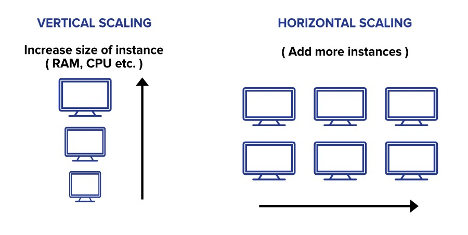
\includegraphics[width=0.8\textwidth]{assets/ScalingAvail.png}
    \caption{Горизонтральное и вертикальное масштабирование}
    \label{fig:Scaling1}
\end{figure}

Стратегии эластичности (elasticity) обеспечивают автоматическое перераспределение ресурсов в зависимости от реальных потребностей. Например, в Kubernetes используются StatefulSets \autocite{StatefulSetsApps} — специальные контроллеры, которые управляют развёртыванием и масштабированием stateful-приложений, обеспечивая уникальные идентификаторы и сохранность данных при масштабировании. 

\begin{figure}[H]
    \centering
    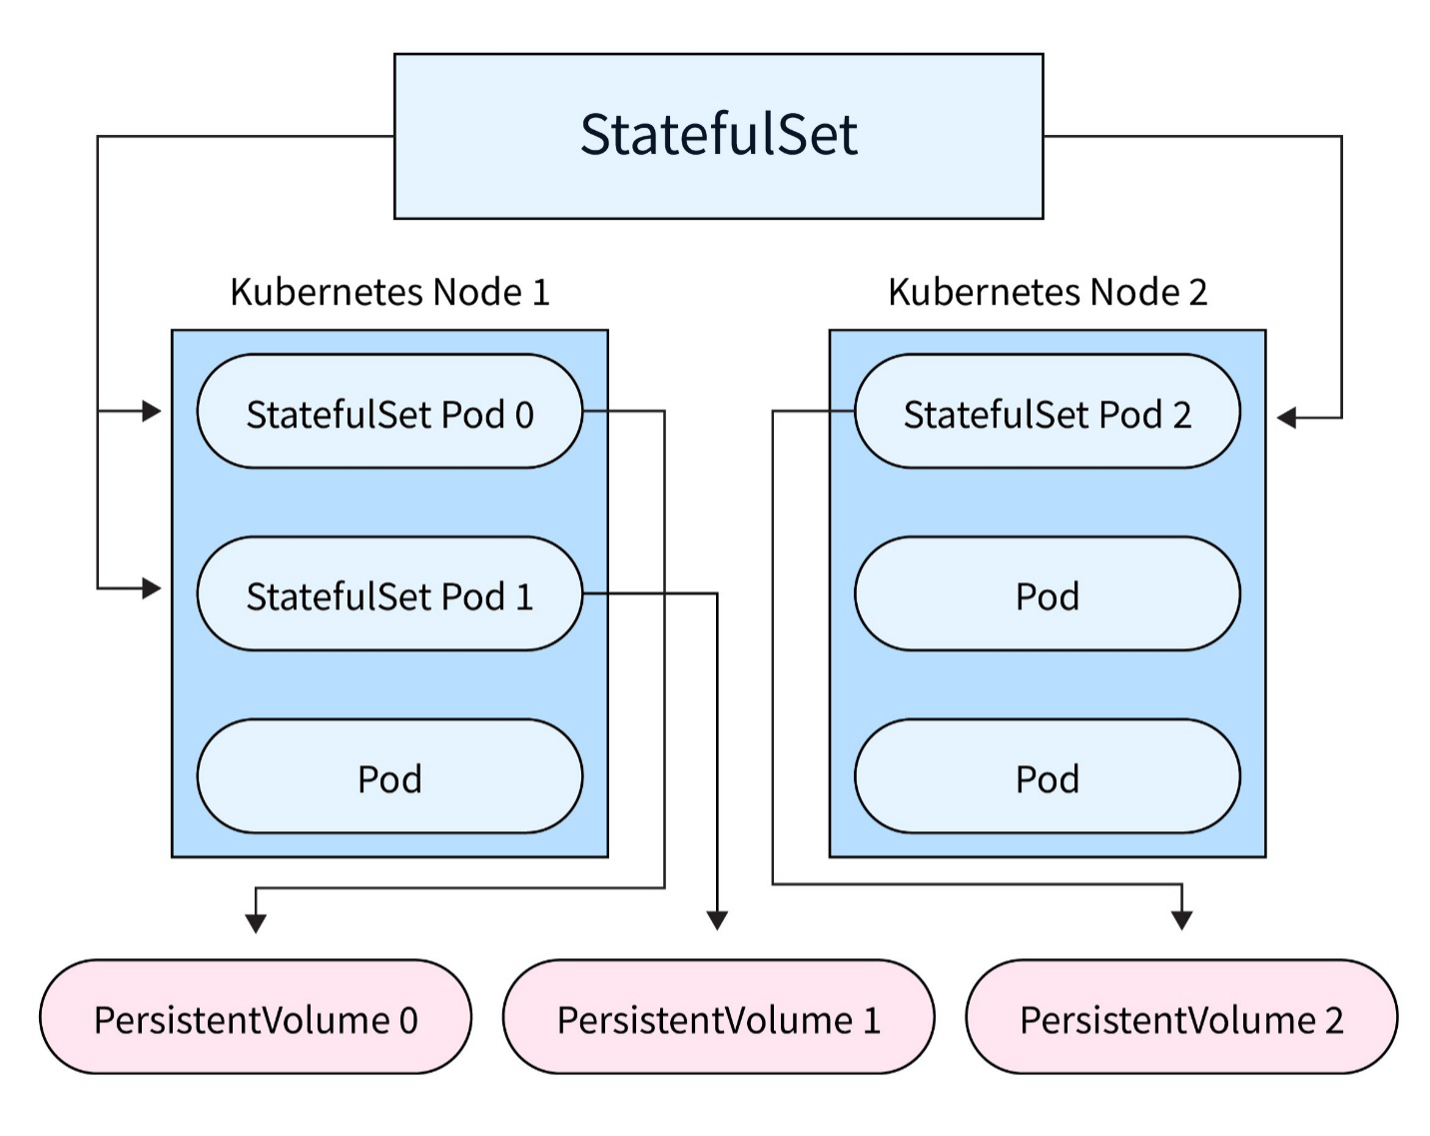
\includegraphics[width=0.8\textwidth]{assets/StatefulSet.png}
    \caption{StatefulSet}
    \label{fig:Scaling2}
\end{figure}

В контексте баз данных, такие решения, как Amazon Aurora Auto Scaling \autocite{AuroraAutoScaling}, автоматически изменяют размер пула реплик в зависимости от нагрузки, гарантируя как производительность, так и высокую доступность при минимальных затратах ресурсов.

\subsection{Системы, обладающие свойством высокой готовности} ~\\

Системы, обладающие свойством высокой готовности (High Availability, HA), представляют собой компонент ИТ-инфраструктуры, обеспечивающий непрерывность бизнес-процессов даже в условиях сбоев или отказов отдельных компонентов. Основной задачей таких систем является минимизация времени простоя и обеспечение устойчивости сервисов к различным видам отказов: от программных ошибок до полного выхода из строя отдельных узлов или даже целых дата-центров.

Высокая готовность достигается путём интеграции различных архитектурных и технологических решений, включающих репликацию, масштабирование, мониторинг, автоматическое восстановление, а также использование устойчивых к сбоям протоколов согласования. Особое внимание уделяется архитектурам распределённых систем, которые обеспечивают гибкость, отказоустойчивость и масштабируемость за счёт децентрализации и избыточности.

\subsubsection{Распределённые базы данных} ~\\

Распределённые СУБД (Distributed Databases) являются частью построения отказоустойчивых систем. За счёт децентрализованного хранения и обработки данных они обеспечивают непрерывность работы сервисов даже при выходе из строя отдельных узлов или сегментов сети. Далее рассмотрим наиболее значимые представители этой категории систем. \autocite{OszuValduriez}

\paragraph{Google Spanner} ~\\

Google Spanner — первая в мире глобально распределённая реляционная СУБД, разработанная Google. Она объединяет свойства реляционных SQL-систем (включая поддержку ACID-транзакций и SQL-запросов) с масштабируемостью NoSQL-решений. В Spanner используется уникальной технологии TrueTime, которая основывается на синхронизации времени через GPS и атомные часы. Это позволяет Spanner достигать глобальной синхронной согласованности и реализовать транзакции с гарантиями линейной согласованности (linearizability) на уровне планетарной масштабируемости. \autocite{Kleppmann}

Система поддерживает автоматическое шардирование и репликацию данных по множеству дата-центров с возможностью выбора уровня согласованности и доступности. Это делает её идеальным решением для критически важных систем, требующих высокой готовности и точности данных, таких как банковские приложения, системы бронирования и глобальные распределённые финансовые платформы.

\paragraph{CockroachDB} ~\\

CockroachDB — это распределённая, транзакционная база данных с открытым исходным кодом, разработанная с прицелом на глобальную доступность и устойчивость к сбоям. Основное вдохновение архитекторы CockroachDB черпали из Google Spanner, однако без необходимости в специализированной аппаратуре вроде TrueTime. Вместо этого она использует протокол консенсуса Raft, позволяющий достичь сильной согласованности при распределённой архитектуре. \autocite{Kleppmann}

CockroachDB совместима с PostgreSQL, это упрощает миграцию и интеграцию с существующими системами. Архитектура <<shared-nothing>> означает, что каждый узел кластера независим и самодостаточен, что исключает единые точки отказа. База данных автоматически распределяет данные по кластерам и реплицирует их с учётом политики отказоустойчивости.

Также присутствует возможность автоматического балансирования нагрузки и переноса данных, а также автоматическое восстановление после сбоя. Кроме того, система поддерживает горизонтальное масштабирование без остановки сервиса, что делает её подходящей для облачных приложений и микросервисной архитектуры.

CockroachDB используется в сферах, где требуется глобальная доступность и транзакционная целостность, включая финтех, e-commerce и IoT-сервисы. Её архитектура делает её устойчивой к целым классам проблем, таких как split-brain, потеря данных при отказе узла и несогласованные транзакции.

\paragraph{YugabyteDB} ~\\

YugabyteDB — это распределённая база данных с открытым исходным кодом, которая совмещает возможности реляционных и нереляционных СУБД. Она поддерживает два основных интерфейса: YSQL — полностью совместимый с PostgreSQL реляционный API, и YCQL — совместимый с Cassandra язык запросов для работы с документами и ключ-значение данными. Такая гибридная модель позволяет YugabyteDB обеспечивать универсальность, оставаясь при этом высокоэффективной в различных сценариях использования.

С точки зрения высокой готовности, YugabyteDB реализует репликацию данных с помощью консенсуса Raft, что обеспечивает сильную согласованность и устойчивость к сбоям. Каждый фрагмент данных (shard) реплицируется между несколькими узлами, и лидерский узел в каждой группе Raft управляет координацией операций. При сбое одного узла кластер автоматически выбирает нового лидера и продолжает работу без вмешательства администратора. \autocite{Choudhury}

YugabyteDB может работать в мультиоблачной среде, с поддержкой геораспределённых кластеров и межрегиональной репликации. Система также поддерживает масштабирование в режиме онлайн без простоев, а также интеграцию с Kubernetes и облачными провайдерами. Это делает YugabyteDB особенно привлекательной для организаций, строящих гибкие, отказоустойчивые и масштабируемые облачные архитектуры.

YugabyteDB находит применение в областях, требующих строгой консистентности и высокой доступности, включая финансовые технологии, цифровую торговлю и IoT-платформы.

\paragraph{Casandra} ~\\
Casandra - распределённая система управления базами данных, относящаяся к классу NoSQL-систем и рассчитанная на создание высокомасштабируемых и надёжных хранилищ огромных массивов данных, представленных в виде хэша \autocite{casandra}. \\
Хранилище само позаботится о проблемах наличия единой точки отказа (single point of failure), отказа серверов и о распределении данных между узлами кластера (cluster node). При чем, как в случае размещения серверов в одном центре обработки данных (data center), так и в конфигурации со многими центрами обработки данных, разделенных расстояниями и, соответственно, сетевыми задержками. Под надёжностью понимается итоговая согласованность (eventual consistency) данных с возможностью установки уровня согласования данных (tune consistency) каждого запроса. \\
Узлы кластера Casandra равноценны, и клиенты могут соединятся с любым из них, как для записи, так и для чтения. Запросы проходят стадию координации, во время которой, выяснив при помощи ключа и разметчика на каких узлах должны располагаться данные, сервер посылает запросы к этим узлам. Будем называть узел, который выполняет координацию — координатором (coordinator), а узлы, которые выбраны для сохранения записи с данным ключом — узлами-реплик (replica nodes). Физически координатором может быть один из узлов-реплик — это зависит только от ключа, разметчика и меток.
Для каждого запроса, как на чтение, так и на запись, есть возможность задать уровень согласованности данных. \\
Когда данные приходят после координации на узел непосредственно для записи, то они попадают в две структуры данных: в таблицу в памяти (memtable) и в журнал закрепления (commit log). Таблица в памяти существует для каждого колоночного семейства и позволяет запомнить значение моментально. Технически это хеш-таблица (hashmap) с возможностью одновременного доступа (concurrent access) на основе структуры данных, называемой “списками с пропусками” (skip list). Журнал закрепления один на всё пространство ключей и сохраняется на диске. Журнал представляет собой последовательность операций модификации. Так же он разбивается на части при достижении определённого размера.
Такая организация позволяет сделать скорость записи ограниченной скоростью последовательной записи на жесткий диск и при этом гарантировать долговечность данных (data durability). Журнал закрепления в случае аварийного останова узла читается при старте сервиса Casandra и восстанавливает все таблицы в памяти. Получается, что скорость упирается во время последовательной записи на диск, а у современных жёстких дисков это порядка 100МБ/с. По этой причине журнал закрепления советуют вынести на отдельный дисковый носитель.

\begin{figure}[h]
    \centering
    \includegraphics[width=0.8\textwidth]{assets/casandra.png}
    \caption{Схема записи в Casandra}
    \label{fig:mesh2}
\end{figure}


\subsubsection{Репликация и согласованность} ~\\

Репликация и согласованность — два основных механизма обеспечения высокой готовности в распределённых системах. Правильно спроектированная стратегия репликации позволяет системе продолжать работу при потере одного или нескольких узлов, а согласованность данных обеспечивает корректность и предсказуемость поведения приложений при доступе к реплицированной информации. \autocite{Kleppmann}

Данный раздел раскрывает основные подходы к репликации — синхронной и асинхронной, обсуждает проблему split-brain и концепцию quorum, а также рассматривает практическое применение данных стратегий на примере популярных систем, таких как etcd, ZooKeeper, Galera Cluster и Pacemaker.

\paragraph{Синхронная и асинхронная репликация} ~\\

В системах с высокой готовностью репликация данных служит основным способом защиты от потери информации и обеспечения непрерывного функционирования. Существует два ключевых подхода к репликации — синхронная и асинхронная — каждый из которых имеет свои преимущества и компромиссы. \autocite{Kleppmann}

Синхронная репликация означает, что данные записываются одновременно на основную и одну или более реплик. Операция считается завершённой только после подтверждения успешной записи со всех задействованных узлов. Это обеспечивает сильную согласованность (strong consistency) и минимизирует риск расхождения данных. Однако синхронная репликация может увеличивать задержки и снижать производительность, особенно в геораспределённых системах.

Асинхронная репликация, напротив, позволяет основной узел завершить транзакцию до того, как изменения будут распространены на реплики. Это уменьшает задержки и увеличивает пропускную способность системы, но создаёт риск потери данных в случае сбоя основного узла до завершения репликации.

Компромисс между этими подходами зависит от специфики приложения: для финансовых и критически важных систем предпочтительнее синхронная репликация, в то время как системы с высокой нагрузкой и требованием минимальной задержки могут использовать асинхронную модель.

\paragraph{Split-brain, CAP-теорема} ~\\

Устойчивость к сетевым сегментациям и способность сохранять согласованность данных необходима при создании распределённых систем высокой готовности. Одним из наиболее опасных сценариев является состояние split-brain — ситуация, при которой кластер делится на несколько частей, не способных коммуницировать между собой. В результате независимые фрагменты системы могут принимать противоречивые решения, что ведёт к несогласованности данных и нарушению бизнес-логики. \autocite{Kleppmann}

Для анализа таких сценариев часто применяется CAP-теорема, согласно которой невозможно одновременно достичь трёх свойств:
\begin{itemize}
    \item \textbf{Consistency (C)} — согласованность: все узлы возвращают одинаковый результат на один и тот же запрос;
    \item \textbf{Availability (A)} — доступность: система всегда отвечает на запросы;
    \item \textbf{Partition tolerance (P)} — устойчивость к разделению: система продолжает работу при разрывах связи между узлами.
\end{itemize}

В условиях реальных отказов системы вынуждены жертвовать либо согласованностью, либо доступностью. Например, Cassandra делает ставку на доступность и устойчивость к разбиению сети, жертвуя строгой согласованностью. Системы, ориентированные на строгую консистентность, наоборот, могут приостанавливать работу части кластера при потере связи.

\paragraph{Quorum} ~\\

Механизм quorum (кворум) широко применяется в распределённых системах для обеспечения согласованности и отказоустойчивости. Кворум — это минимальное количество узлов, которые должны участвовать в принятии решения, чтобы оно считалось валидным. Использование кворума позволяет системам достичь баланса между доступностью и согласованностью при наличии сбоев. \autocite{Kleppmann}

Существует два основных типа операций с кворумом:
\begin{itemize}
    \item \textbf{Quorum-запись (write quorum)} — операция записи считается успешной только после подтверждения от достаточного числа реплик (обычно более половины).
    \item \textbf{Quorum-чтение (read quorum)} — операция чтения выполняется с достаточного количества реплик, чтобы гарантировать возврат актуальных данных, даже если не все реплики синхронизированы.
\end{itemize}

Простое правило: если сумма долей узлов, участвующих в чтении и записи, превышает общее количество реплик, система может обеспечить strong consistency. Например, при трёх репликах quorum-чтение и quorum-запись требуют ответов минимум от двух узлов.

Механизм quorum предотвращает split-brain и обеспечивает устойчивость к отказу отдельных компонентов. Он используется во многих СУБД и системах управления конфигурациями, включая Cassandra, etcd, ZooKeeper и Galera Cluster.

\paragraph{Примеры систем репликации и согласованности} ~\\

Ряд широко используемых программных решений реализует принципы репликации и согласованности, обеспечивая основу для построения отказоустойчивых и консистентных распределённых систем. Эти инструменты применяются как в базах данных, так и в кластерных конфигурациях различных приложений.

\begin{itemize}
    \item \textbf{etcd} — распределённое хранилище ключ-значение с открытым исходным кодом, разработанное как часть Kubernetes. etcd использует алгоритм консенсуса Raft для обеспечения согласованности данных. Он широко применяется для хранения конфигураций и обнаружения сервисов, а также обеспечивает высокую доступность и автоматическое восстановление после сбоев. \autocite{Kleppmann}
    \item \textbf{ZooKeeper} — централизованный сервис для координации распределённых приложений. Он реализует журнал транзакций, поддерживает очереди, блокировки и обеспечивает согласованность данных. Используется многими системами (включая Apache Kafka, HBase и Hadoop) для управления конфигурацией и координации кластеров. \autocite{Kleppmann}
    \item \textbf{Galera Cluster} — решение для синхронной мульти-мастер репликации в MySQL и MariaDB. Все узлы в кластере равноправны, и изменения применяются ко всем репликам одновременно. Это гарантирует strong consistency и предотвращает конфликтные изменения. Поддерживает автоматическое переключение узлов и масштабирование на чтение. \autocite{GaleraCl}
    \item \textbf{Pacemaker} — кластерный менеджер, используемый в высокодоступных конфигурациях на уровне операционной системы и сервисов. Он управляет состоянием ресурсов, отслеживает здоровье узлов, выполняет автоматический failover и интегрируется с такими решениями, как Corosync и DRBD. Pacemaker широко используется в HA-кластерах для приложений и БД. \autocite{Sosemkaram}
\end{itemize}


\subsubsection{Программные платформы обеспечения высокой готовности} ~\\

Помимо архитектуры и основных принципов распределённых систем управления базами данных, значительное значение для обеспечения высокой доступности имеют программные платформы, которые автоматизируют процессы репликации, смены ролей, мониторинга состояния кластера и восстановления после сбоев. Ниже представлены решения, применяемые в системах на базе PostgreSQL, MySQL и MariaDB.

\paragraph{PostreSQL + Patroni} ~\\

Patroni — это Python-приложение для создания высокодоступных PostgreSQL кластеров на основе потоковой репликации. С его помощью можно преобразовать систему из ведущего и ведомых узлов (primary — replica) в высокодоступный кластер с поддержкой автоматического контролируемого (switchover) и аварийного (failover) переключения. Patroni позволяет легко добавлять новые реплики в существующий кластер, поддерживает динамическое изменение конфигурации PostgreSQL одновременно на всех узлах кластера и множество других возможностей, таких как синхронная репликация, настраиваемые действия при переключении узлов, REST API, возможность запуска пользовательских команд для создания реплики вместо pg basebackup, взаимодействие с Kubernetes и т.д. \autocite{Klyukin} \\

Опишем, как используется Patroni. Сама по себе потоковая репликация не является достаточным средством обеспечения высокой доступности. Потому что нет никакого встроенного решения, которое бы позволило перевести standby в режим нового мастера, если что-то произошло со старым мастером. Рассмотрим на примере \autocite{Aristov}.\\
Возьмем кластер из двух нод, и, допустим, у нас есть программа, запущенная на standby-сервере, мониторящая, жив ли основной сервер, и при его падении повышающая реплику до основного сервера:

\begin{figure}[h]
    \centering
    \includegraphics[width=0.8\textwidth]{assets/Patroni1.png}
    \caption{Кластер из двух нод}
    \label{fig:mesh3}
\end{figure}

Вроде всё хорошо, но что произойдёт, если у нас просто случится обрыв сетевого подключения между серверами?

\begin{figure}[h]
    \centering
    \includegraphics[width=0.8\textwidth]{assets/Patroni2.png}
    \caption{Кластер из двух нод}
    \label{fig:mesh4}
\end{figure}

Правильно! Получим два независимых основных кластера, каждый из них будет принимать запросы на запись, и мы получим такую ситуацию:

\begin{figure}[h]
    \centering
    \includegraphics[width=0.8\textwidth]{assets/Patroni3.png}
    \caption{Разрыв соединения в кластере из двух нод}
    \label{fig:mesh5}
\end{figure}

Она называется splitbrain. Это очень плохая ситуация, и в дальнейшем объединить изменённые данные с двух независимых серверов без потерь практически нереально.
Казалось бы, есть простое решение - добавить стороннего наблюдателя.
Что же может пойти не так в данной конфигурации:

\begin{figure}[h]
    \centering
    \includegraphics[width=0.8\textwidth]{assets/Patroni4.png}
    \caption{Кластер из двух нод со сторонним наблюдателем}
    \label{fig:mesh6}
\end{figure}

В такой конфигурации могут возникнуть две проблемы: во-первых, может умереть наблюдатель и мониторить станет некому, во-вторых, может оборваться соединение с основной нодой и опять мы получаем splitbrain. 

И Patroni предлагает решение данной проблемы - это использование отказоустойчивого кластера для наблюдателя, в котором мы будем хранить статус активного сервера. То есть основной будет активно ходить и поддерживать статус основного, а остальные будут опрашивать жив ли основной сервер. При потере с ним соединения через некоторое время произойдут выборы и вторичный сервер станет основным и будет активно поддерживать свой статус в этом отказоустойчивом наблюдателе. При этом изначальный основной сервер при недоступности кластера наблюдения перейдёт в статус “только чтение".

\begin{figure}[h]
    \centering
    \includegraphics[width=0.8\textwidth]{assets/Patroni5.png}
    \caption{Решение, используемое в Patroni}
    \label{fig:mesh7}
\end{figure}

Quorum позволяет нам решать сложные задачи разрешения партицирования сети. Когда какой-то сегмент сети недоступен, то несколько других сегментов могут принимать решения. А изолированный сегмент в этом случае должен остановить старого мастера. 

\paragraph{Orchestrator} ~\\
Orchestrator — это инструмент с открытым исходным кодом, предназначенный для управления топологией кластеров MySQL и MariaDB. Он позволяет визуализировать структуру репликации, автоматически обнаруживать изменения в топологии, мониторить состояние узлов и выполнять автоматические или ручные операции failover и recovery. \autocite{Openarc}

Orchestrator позволяет автоматическое переключение на новый ведущий узел в случае сбоя текущего. При этом учитываются приоритеты реплик, их «запаздывание» (replication lag) и доступность, что позволяет избежать выбора неактуальной или перегруженной реплики. Система обеспечивает безопасное и последовательное переназначение репликации с минимальной потерей доступности.

Orchestrator умеет строить топологию на лету, включая поддержку сложных деревьев репликации и циклов. Он предоставляет веб-интерфейс для визуального контроля над структурой кластера и CLI/HTTP API для автоматизации операций. Также поддерживается интеграция с внешними инструментами, включая ProxySQL, Consul, HAProxy и системы управления конфигурацией.

Для обеспечения высокой готовности Orchestrator часто используется в связке с сторожевыми службами (watchdog), которые отслеживают его рекомендации и принимают решение о переключении IP-адресов, уведомлении администраторов и запуске сопутствующих сценариев восстановления.

Система активно применяется в продакшене крупными компаниями (GitHub, Booking.com, Zalando) и зарекомендовала себя как устойчивое решение для обеспечения отказоустойчивости в масштабируемых кластерах MySQL.

\paragraph{Galera Cluster} ~\\
Galera Cluster — это высокодоступное решение для синхронной мульти-мастер репликации в системах управления базами данных MySQL, MariaDB и Percona XtraDB. Основное преимущество Galera заключается в том, что все узлы кластера равноправны и могут выполнять как операции чтения, так и записи. Это отличает его от распространенных схем с одним ведущим узлом и множеством ведомых реплик. \autocite{GaleraCl}

Galera реализует синхронную репликацию на уровне транзакций: перед фиксацией (commit) изменения согласуются со всеми активными узлами через внутренний протокол Group Communication System (GCS). Это обеспечивает strong consistency — все узлы всегда находятся в согласованном состоянии, и вероятность конфликта или потери данных минимальна.

Дополнительные особенности:
\begin{itemize}
    \item Автоматическое восстановление: при сбое одного из узлов кластер продолжает работу, а при возвращении узел догоняет актуальное состояние без участия администратора.
    \item Автоматическое добавление новых узлов: для масштабирования не требуется ручная настройка репликации.
    \item Масштабирование на чтение: все узлы обслуживают запросы чтения, что значительно увеличивает производительность при высокой нагрузке.
\end{itemize}

Galera активно используется в системах, где критически важны отказоустойчивость и точность транзакций, например, в телекоммуникационных сервисах, банковской отрасли и высоконагруженных веб-платформах. Благодаря простоте развертывания и гибкости конфигурации Galera является одним из самых популярных решений для построения HA-кластеров на базе MySQL и его производных.

\paragraph{Инфраструктура хранения и акселерация} ~\\
В системах с высокой степенью готовности подсистема хранения данных имеет большое значение, так как она гарантирует отказоустойчивость, постоянный доступ к данным и оперативное восстановление информации. Ошибки в подсистеме хранения способны привести к полной недоступности сервисов, даже если вычислительные и сетевые компоненты функционируют нормально. По этой причине архитектуры хранения данных в HA-системах проектируются с избыточностью, масштабируемостью и поддержкой высокопроизводительных протоколов ввода-вывода. \autocite{SnedakerS}

Современные подходы к построению отказоустойчивой инфраструктуры хранения включают использование скоростных интерфейсов доступа, гибких архитектур хранения и аппаратных ускорителей обработки данных. Эти технологии снижают задержки при доступе к данным, обеспечивают высокую пропускную способность и повышают отказоустойчивость всей платформы.

\paragraph{NVMe и NVMe-over-Fabrics (NVMe-oF)} ~\\
NVMe (Non-Volatile Memory Express) — это высокопроизводительный интерфейс доступа к энергонезависимым твердотельным накопителям, разработанный с целью преодоления ограничений классических протоколов ввода-вывода, таких как SATA и SAS. Основное преимущество NVMe заключается в эффективной работе с параллельными потоками операций, благодаря чему достигается значительное снижение задержек и рост производительности. \autocite{Nvme}

NVMe использует шину PCI Express (PCIe), позволяя передавать команды напрямую в контроллер накопителя с минимальным вмешательством центрального процессора. Это обеспечивает высокую плотность операций ввода-вывода (IOPS), критически важную для систем, обрабатывающих большое количество транзакций в реальном времени — таких как базы данных, OLTP-системы и системы сбора телеметрии.

NVMe-over-Fabrics (NVMe-oF) представляет собой развитие базовой технологии NVMe, позволяя использовать её преимущества в сетевых средах. В отличие от локального интерфейса PCIe, NVMe-oF передаёт команды и данные через высокоскоростные сетевые интерфейсы, такие как RDMA over Converged Ethernet (RoCE), TCP и Fibre Channel. Это позволяет объединять хранилища в масштабируемые отказоустойчивые архитектуры, обеспечивая при этом близкие к локальным накопителям характеристики задержек и пропускной способности. \autocite{Nvmeof}

Преимущества NVMe и NVMe-oF в контексте высокой готовности:
\begin{itemize}
    \item Минимизация задержек — критично для обеспечения быстрого отклика сервисов.
    \item Горизонтальное масштабирование — хранилище можно увеличивать без простоев и перераспределения нагрузки.
    \item Повышенная отказоустойчивость — благодаря сетевой топологии и возможности многопутевого доступа (multipathing).
    \item Гибкость конфигурации — NVMe-oF может быть интегрирована с существующими архитектурами SAN и кластерными системами хранения.
\end{itemize}

\paragraph{Архитектуры хранения: SAN, NAS и DAS} ~\\
Инфраструктура хранения в высокодоступных системах может реализовываться в различных архитектурных вариантах в зависимости от требований к производительности, масштабируемости и устойчивости к сбоям. Наиболее распространённые подходы — это Direct Attached Storage (DAS), Network Attached Storage (NAS) и Storage Area Network (SAN). Каждая из архитектур обладает своими преимуществами и ограничениями, что делает её более или менее подходящей для конкретных сценариев эксплуатации. \autocites{SnedakerS}{WallaceWebber}

\begin{itemize}
    \item Direct Attached Storage (DAS) представляет собой устройства хранения, напрямую подключённые к конкретному серверу через интерфейсы SATA, SAS или PCIe. DAS обеспечивает низкую задержку доступа и высокую скорость ввода-вывода, но лишён механизмов совместного доступа и масштабирования. Его использование оправдано в системах с локализованными вычислениями, где надёжность обеспечивается на уровне сервера или приложения.
    \item Network Attached Storage (NAS) предоставляет файловый доступ к данным по сети, используя протоколы NFS, SMB/CIFS и др. Основное преимущество NAS — централизованное управление и упрощённый совместный доступ к данным. Однако пропускная способность и задержки зависят от состояния сети, что делает NAS менее подходящим для высоконагруженных транзакционных систем, но полезным в качестве резервного или вспомогательного хранилища.
    \item Storage Area Network (SAN) реализует блочный доступ к данным через выделенную высокоскоростную сеть (обычно Fibre Channel или iSCSI). Это наиболее производительная и масштабируемая архитектура хранения, применяемая в критически важных системах, где требуется высокая отказоустойчивость, минимальные задержки и возможность горячего переключения ресурсов при сбоях. SAN поддерживает технологии зеркалирования, снапшотов, мультипутизации и резервирования на уровне контроллеров и сетей.
\end{itemize}

\paragraph{Аппаратная акселерация: FPGA, SmartNICs и Exadata} ~\\
Повышение отказоустойчивости и производительности на уровне хранения данных требует не только архитектурных решений, но и применения специализированных аппаратных ускорителей. Эти технологии позволяют минимизировать задержки, повысить пропускную способность и реализовать адаптивное управление потоками данных. Наиболее перспективные направления в этом контексте — использование FPGA, SmartNICs и комплексных решений уровня Exadata.

\begin{itemize}
    \item FPGA (Field-Programmable Gate Arrays) представляют собой перепрограммируемые логические интегральные схемы, которые позволяют реализовать специализированные алгоритмы обработки данных прямо в оборудовании. Это обеспечивает сверхнизкие задержки, высокую параллельность обработки и возможность адаптации под конкретные задачи, включая компрессию, дедупликацию, шифрование и управление трафиком хранения. В инфраструктуре HA FPGA часто используются в высокоскоростных каналах передачи данных между узлами и для предварительной фильтрации данных на периферии (edge processing). \autocite{Dutta}
    \item SmartNICs (Smart Network Interface Cards) — интеллектуальные сетевые карты, содержащие встроенные процессоры, FPGA или SoC (System-on-Chip). Они разгружают центральный процессор сервера, выполняя функции маршрутизации, балансировки нагрузки, шифрования и протоколирования на аппаратном уровне. В контексте высокой готовности SmartNICs позволяют значительно повысить пропускную способность сети и минимизировать время обработки пакетов, особенно в кластерах с распределённым доступом к хранилищу. \autocite{Alshahrani}
    \item Oracle Exadata — комплексная программно-аппаратная платформа для высокопроизводительной обработки и хранения данных. Она включает в себя интеграцию мощных вычислительных узлов, твердотельных накопителей (Flash Cache), сетей InfiniBand и специализированных алгоритмов оптимизации запросов Oracle Database. Exadata поддерживает масштабируемую архитектуру с резервированием компонентов, автоматическое перераспределение нагрузки и самовосстановление после сбоев, что делает её эталонной платформой HA-класса для крупных корпоративных СУБД. \autocite{Exadata}
\end{itemize}

\subsection{Практические кейсы и ограничения} ~\\

Разработка и внедрение архитектур с высокой готовностью требует не только теоретического понимания принципов отказоустойчивости, но и опоры на практический опыт масштабных распределённых систем. В реальных условиях такие системы неизбежно сталкиваются с ограничениями, компромиссами и непредвиденными отказами, которые невозможно воспроизвести в лабораторной среде. По этой причине практические кейсы и методы эмпирической верификации устойчивости становятся важнейшими источниками инженерного знания.

Компании, эксплуатирующие крупномасштабные распределённые инфраструктуры, такие как Facebook, Netflix и Google, разработали собственные стратегии обеспечения высокой доступности, адаптированные к требованиям конкретных рабочих нагрузок. Эти подходы сочетают масштабирование, репликацию, автоматическое восстановление и устойчивые протоколы согласования. В дополнение к архитектурным решениям, всё более важное значение приобретают методы активного тестирования отказов в продуктивных средах, получившие название \textit{chaos engineering}.

Кроме инженерных решений, практическая реализация HA-систем выявляет ряд ограничений: временные задержки при переключении ролей, угрозу split-brain, сложность валидации поведения при отказах и необходимость баланса между доступностью и согласованностью. Эти ограничения формируют требования к организационным процессам, инженерной культуре и средствам автоматизации, то есть не являются исключительно техническими.

\subsubsection{Кейсы из реального мира} ~\\

\paragraph{Масштабируемость и отказоустойчивость через шардирование (Facebook)} ~\\

Facebook использует масштабируемую архитектуру хранения данных, основанную на модифицированной версии MySQL, адаптированной для работы в условиях высокой нагрузки и необходимости горизонтального масштабирования. Ключевым компонентом этой архитектуры является система Shard Manager, разработанная для управления шардированием, балансировкой нагрузки и отказоустойчивостью \autocite{FBShardManager}.

Shard Manager обеспечивает автоматическое распределение шардов по серверам, динамическую балансировку нагрузки и управление репликацией. Он поддерживает различные типы приложений, включая те, которые требуют строгой согласованности данных и высокой доступности. Система позволяет масштабировать приложения, управляя миллионами шардов на сотнях тысяч серверов.

Для обеспечения высокой доступности и отказоустойчивости Facebook использует геораспределённую репликацию данных. Ранее применялась полусинхронная репликация MySQL, при которой основная база данных использовала два логических репликатора для подтверждения записи данных. Это обеспечивало низкую задержку при записи и высокую надёжность. Впоследствии была внедрена система MySQL Raft, основанная на протоколе Raft, для улучшения согласованности и управления репликацией \autocite{FBRaftMeta}.

Кроме того, Facebook разработал систему TAO для эффективного доступа к социальному графу. TAO использует шардированную архитектуру на основе MySQL, где каждый шард представляет собой логическую базу данных с таблицами для объектов и их ассоциаций. Это позволяет масштабировать хранение и обработку данных, обеспечивая высокую производительность и отказоустойчивость \autocite{TAODistributedGraph}.

В общем говоря, архитектура хранения данных Facebook основана на сочетании шардирования, геораспределённой репликации и специализированных систем управления. И это обеспечивает высокую масштабируемость и устойчивость к отказам в условиях глобальной инфраструктуры.

\paragraph{Chaos Engineering (Netflix)} ~\\

Netflix стал одним из первых крупных технологических гигантов, внедривших практику целенаправленного тестирования отказоустойчивости — подход, получивший название \textit{chaos engineering}. Этот метод предполагает преднамеренное внесение сбоев в систему для оценки её устойчивости в условиях реальных эксплуатационных отказов.

Центральным инструментом Netflix в этой области стал \textit{Chaos Monkey} — сервис, разработанный в рамках инициативы \textit{Simian Army}. Chaos Monkey случайным образом выключает экземпляры сервисов, имитируя реальные сбои, с целью проверки способности системы к автоматическому восстановлению без вмешательства операторов \autocite{NetflixSimianArmy}.

Помимо отдельных сбоев, Netflix моделирует более сложные сценарии: отказов целых зон доступности, деградацию сетей, перегрузки отдельных компонентов. Для этого применяются расширенные инструменты \textit{Chaos Gorilla} и \textit{Latency Monkey}. Такой подход позволяет выявлять уязвимости архитектуры, которые могли бы остаться незамеченными в условиях нормальной эксплуатации.

\textit{Chaos Engineering} в Netflix стал частью производственного цикла. Принципиальной особенностью является запуск отказов в продуктивной среде, что позволяет моделировать поведение в максимально приближённых к реальности условиях, при этом минимизируя риски с помощью заранее заданных границ экспериментов.

Успех Netflix в этой области оказал значительное влияние на индустрию, и принципы \textit{Chaos Engineering} были переняты другими организациями, включая Microsoft, Google и Shopify. В Kubernetes-среде аналогичные практики реализуются с помощью фреймворков \textit{LitmusChaos} и \textit{Chaos Mesh} \autocites{LitmusChaosIntro}{ChaosMeshDocs}.

\paragraph{Google: глобальная архитектура высокой готовности} ~\\

Инфраструктура Google строится с приоритетом на масштабируемость, устойчивость к отказам и глобальную доступность. Ключевую роль в обеспечении этих свойств играет архитектура распределённых систем, в первую очередь — Google Spanner, используемый в качестве внутренней и облачной платформы для хранения критически важных данных.

Google Spanner сочетает свойства реляционных баз данных (поддержка SQL и транзакций ACID) с масштабируемостью и отказоустойчивостью распределённых NoSQL-систем. В основе Spanner лежит протокол консенсуса Paxos и уникальная система синхронизации времени TrueTime, которая использует GPS и атомные часы для достижения глобальной согласованности (linearizability) между географически удалёнными дата-центрами \autocite{Corbett}.

Система Spanner обеспечивает автоматическое шардирование и синхронную репликацию данных по нескольким регионам, что позволяет выполнять транзакции с высокой степенью устойчивости даже при выходе из строя целых зон доступности. Она применяется в таких сервисах, как Google Ads, Google Play и Gmail, где сбои и задержки недопустимы на уровне пользовательского опыта.

На уровне оркестрации инфраструктуры Google использует систему Borg, предшественник Kubernetes. Borg управляет размещением и восстановлением контейнеризованных сервисов в распределённой среде. Вместе с Spanner и системами мониторинга, такими как Dapper и Monarch, это позволяет Google реализовывать полную автоматизацию отказоустойчивости: от балансировки нагрузки до детектирования и устранения сбоев в реальном времени \autocite{GoogleDremel}.

Подход Google показывает, как жесткие инженерные решения, опирающиеся на формальные свойства алгоритмов и точность времени, помогают построения сервисов, работающих в масштабе планеты с практически нулевым временем простоя.

\subsubsection{Потенциальные проблемы высокой готовности}

\paragraph{Задержки при failover} ~\\

Один из ключевых факторов высокой готовности информационных систем — минимизация времени восстановления после сбоя (Recovery Time Objective, RTO). Несмотря на широкое применение репликации и механизмов автоматического переключения на резервные узлы, задержки, возникающие на этапах обнаружения отказа, выбора нового ведущего узла и перенастройки клиентских соединений, по-прежнему остаются значимым препятствием на пути к снижению общего времени простоя \autocite{USENIXLi}.

Особенно выражены эти задержки в системах с высокой нагрузкой и жёсткими требованиями к согласованности. В классических подходах, таких как Raft и Paxos, переключение роли лидера требует достижения кворума, что может быть затруднено в условиях сетевых сбоев или деградации производительности. Кроме того, асинхронная репликация, хотя и обеспечивает низкую латентность, порождает риск рассогласования данных, требующий дополнительной логики восстановления.

Дополнительную проблему представляет тот факт, что failover-процедуры нередко выполняются последовательно: сначала осуществляется подтверждение отказа, затем начинается восстановление состояния на резервном узле. Такой подход характерен, например, для архитектур на основе разобщённого хранения (REDS). В этих системах диск должен быть отсоединён от потенциально неисправного узла до начала процедуры восстановления, что ведёт к задержке, обусловленной таймаутом ожидания. В некоторых конфигурациях, таких как Kubernetes, он может достигать нескольких минут.

Современные подходы к снижению задержек при failover предполагают параллелизацию процессов детектирования отказа и восстановления. Один из таких механизмов — спекулятивное восстановление (speculative recovery), при котором система немедленно запускает восстановление на резервном узле с использованием копии хранилища, не дожидаясь окончательного подтверждения недоступности основного. Если основной узел восстанавливает работоспособность раньше, резервный процесс останавливается, а состояние возвращается к первичной конфигурации. Такой подход позволяет существенно сократить общее время переключения и минимизировать простои, не нарушая согласованности состояния системы.

То есть даже при наличии эффективных алгоритмов консенсуса и репликации, временные характеристики failover остаются важным инженерным вызовом. Их минимизация требует комбинирования надёжных протоколов обнаружения, оптимизированных механизмов восстановления и архитектурных решений, допускающих спекулятивное или предварительное резервирование ресурсов.

\paragraph{Split-brain} ~\\

В распределённых системах высокой готовности одним из наиболее критичных сбоев является ситуация split-brain — состояние, при котором несколько узлов кластера одновременно считают себя активными и продолжают обслуживать запросы, не осознавая существования других активных узлов. Это приводит к рассогласованию данных, нарушению согласованности и потенциальной потере информации.

Split-brain обычно возникает в результате сетевой сегментации (network partition), когда узлы теряют возможность обмениваться heartbeat-сообщениями. В отсутствие надёжного механизма согласования каждый сегмент кластера может принять решение о самостоятельной активации, полагая, что остальные узлы недоступны. Подобные сценарии особенно опасны в архитектурах с активной репликацией или при использовании общего хранилища, где параллельная запись данных разными узлами может привести к их повреждению \autocite{SplitBrainEtcd}.

Для предотвращения split-brain применяются различные подходы. Одним из наиболее эффективных является использование кворума — механизма, при котором только та часть кластера, которая обладает большинством голосов, может продолжать работу. Это достигается посредством внедрения дополнительных компонентов, таких как witness-узлы или quorum-диски, которые обеспечивают арбитраж в случае сетевых сбоев. Например, в двухузловых кластерах добавление третьего узла, выполняющего роль свидетеля, позволяет избежать ситуаций, при которых оба основных узла одновременно становятся активными.

Альтернативным методом является использование pessimistic fencing — стратегии, при которой в случае потери связи узел автоматически переходит в пассивное состояние до восстановления полной связности. Это обеспечивает сохранение согласованности данных за счёт временного снижения доступности. В некоторых системах реализуются гибридные подходы, сочетающие кворум и автоматическое отключение узлов, не прошедших проверку.

\paragraph{Тестирование отказов} ~\\

Тестирование отказов является неотъемлемой частью обеспечения надёжности и устойчивости распределённых систем. В условиях высокой сложности и взаимодействия множества компонентов, традиционные методы тестирования зачастую оказываются недостаточными для выявления скрытых уязвимостей. Для преодоления этих ограничений был разработан подход, известный как \textit{Chaos Engineering}, который предполагает преднамеренное внесение сбоев в систему с целью изучения её поведения и выявления потенциальных точек отказа \autocite{GremlinChaosEngineering}.

\textit{Chaos Engineering} основывается на проведении контролируемых экспериментов, в ходе которых в систему вводятся различные виды сбоев, такие как отключение узлов, увеличение задержек, потеря пакетов или отказ внешних зависимостей. Целью этих экспериментов является проверка способности системы сохранять работоспособность и обеспечивать требуемый уровень обслуживания в условиях непредвиденных ситуаций. Принципы \textit{Chaos Engineering} включают формулирование гипотез о поведении системы, проведение экспериментов в максимально приближенных к реальным условиям и анализ результатов для выявления и устранения уязвимостей.

Одним из ключевых аспектов \textit{Chaos Engineering} является возможность проведения тестов в производственной среде, что позволяет получить наиболее достоверные данные о поведении системы под нагрузкой. Однако это требует тщательного планирования и ограничения области воздействия экспериментов, чтобы минимизировать потенциальные риски для пользователей. Практика проведения таких экспериментов, известная как \textit{GameDay}, позволяет командам отработать сценарии отказов и улучшить процессы реагирования на инциденты.

Современные инструменты для тестирования отказов, такие как \textit{Gremlin}, \textit{Chaos Monkey} и другие, предоставляют возможности для автоматизации и упрощения процесса проведения экспериментов. Эти инструменты позволяют моделировать различные сценарии сбоев и анализировать поведение системы в реальном времени, что способствует повышению её устойчивости и надёжности.

\paragraph{Баланс CAP-теоремы} ~\\

CAP-теорема, сформулированная Эриком Брюером в 2000 году и формально доказанная Сетом Гилбертом и Нэнси Линч в 2002 году, утверждает, что в условиях сетевой сегментации (partition) распределённая система может гарантировать одновременно только два из трёх свойств: согласованность (Consistency), доступность (Availability) и устойчивость к разделению сети (Partition Tolerance). Это означает, что при проектировании распределённых систем необходимо делать осознанный выбор в пользу двух из этих свойств, жертвуя третьим \autocite{CAPTheoremGeeks}.

В условиях неизбежности сетевых разделений, большинство практических систем стремятся обеспечить устойчивость к разделению сети, что приводит к необходимости выбора между согласованностью и доступностью. Системы, ориентированные на согласованность (CP-системы), при возникновении разделения сети могут стать недоступными для обеспечения целостности данных. Примеры таких систем включают традиционные реляционные базы данных и распределённые файловые системы с жёсткими требованиями к консистентности. С другой стороны, системы, ориентированные на доступность (AP-системы), продолжают обслуживать запросы даже при разделении сети, что может привести к временной несогласованности данных. Примеры таких систем включают NoSQL-базы данных, такие как Cassandra и DynamoDB \autocite{CAPTheoremIBM}.

Для более точного описания компромиссов в распределённых системах была предложена теорема PACELC, расширяющая CAP-теорему. Согласно PACELC, даже при отсутствии разделения сети (Else), необходимо выбирать между задержкой (Latency) и согласованностью (Consistency). Это подчёркивает, что компромиссы между задержкой и согласованностью актуальны не только при сетевых сбоях, но и в нормальных условиях работы системы.

Для проектирования надёжных и масштабируемых распределённых систем нужно понимание и применение CAP-теоремы и её расширений. Выбор между согласованностью, доступностью и устойчивостью к разделению сети должен основываться на специфике приложения, требованиях к данным и ожидаемых условиях эксплуатации системы.
